% !TeX spellcheck = es_ES
% Chapter 1

%\chapter{Chapter Title Here} % Main chapter title
%
%\label{Chapter1} % For referencing the chapter elsewhere, use \ref{Chapter1} 

%----------------------------------------------------------------------------------------

% Define some commands to keep the formatting separated from the content 
%\newcommand{\keyword}[1]{\textit{#1}}
%\newcommand{\tabhead}[1]{\textbf{#1}}
%\newcommand{\code}[1]{\texttt{#1}}
%\newcommand{\file}[1]{\texttt{\bfseries#1}}
%\newcommand{\option}[1]{\texttt{\itshape#1}}

%----------------------------------------------------------------------------------------

\chapter{Control de la temperatura}
	El sistema cuenta con dos calentadores de precisión al interior del baño termostatado de 25 litros. Estos calentadores junto con el ba\~no externo determinan la temperatura de trabajo del equipo. El ba\~no externo se usa con el objetivo de mantener siempre activos los calentadores internos en alg\'un nivel de potencia intermedio, pues el ba\~no externo, al tener una temperatura inferior agregar una carga permanente a los calentadores internos \cite{Suurkuusk}. Para monitorear la temperatura del ba\~no el calor\'imetro cuenta con dos termistores, el primero para trabajar a temperaturas inferiores a 50 $^\circ$C y el segundo para temperaturas superiores a este valor. La se\~nal generada por uno de estos termistores se compara con un valor de resistencia definido por el usuario. La resistencia y por ende la temperatura del equipo se fijan usando cuatro resistencias de década, esto es que cada resistencia es una potencia de 10 menor que la anterior, las cuales se encuentran en la parte inferior del calor\'imetro (\autoref{fig: decadeResistors}), de esta manera se pueden realizar experimentos a temperaturas en el rango de 5 a 80 $^\circ$C. El diagrama del sistema de control t\'ermico del calor\'imetro se muestra en el \autoref{ch: anexos} como \autoref{fig: controlTermico}.
	
	\begin{figure}[h]
		\centering
		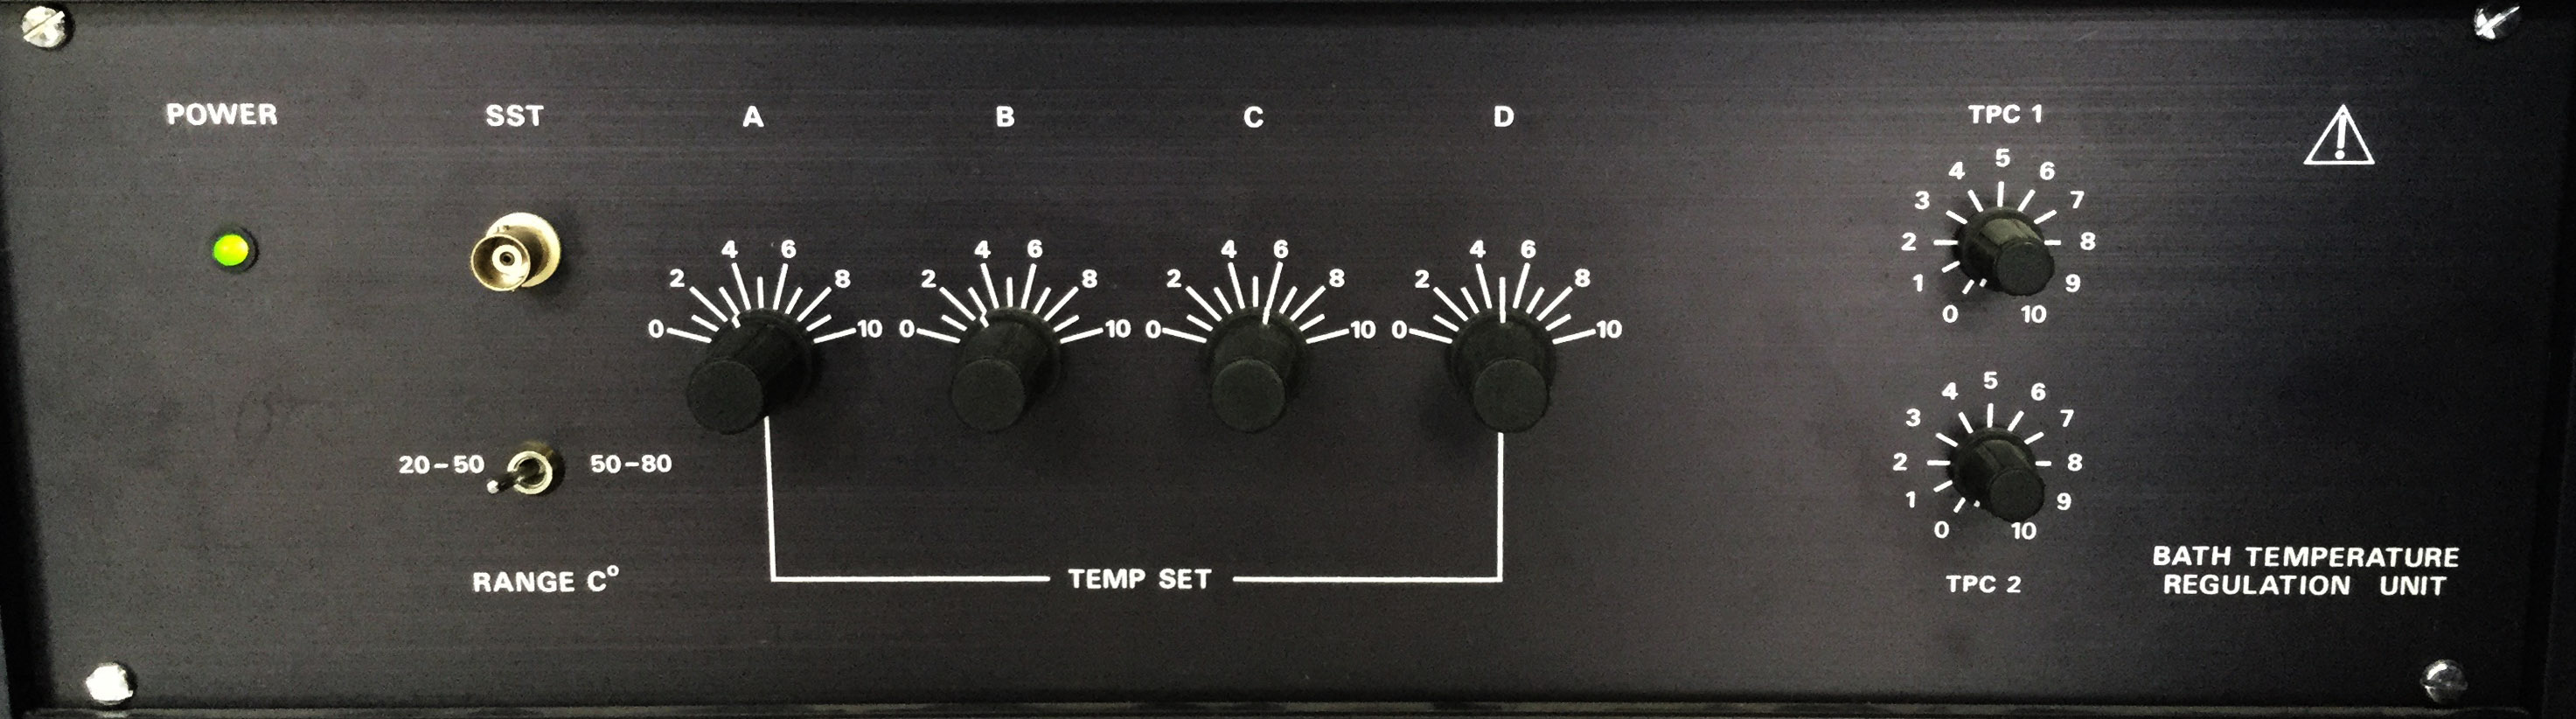
\includegraphics[width=\linewidth]{Figures/decadeResistors}
		\caption{Resistencias de década que controlan la temperatura.}
		\label{fig: decadeResistors}
	\end{figure}
	
	Para determinar la equivalencia de resistencia y temperatura el calorímetro cuenta con una tabla que relaciona los valores de resistencia y temperatura de ba\~no externo que dan lugar a una temperatura constante en el ba\~no interno. Dicha tabla se muestra en el \autoref{ch: anexos} como \autoref{fig: temperatureTable}, sin embargo, el uso de esa tabla est\'a limitado a temperaturas ambiente superiores a 20 $^\circ$C por lo cual, en el caso particular de Bogot\'a rara vez se cumplen. Lo anterior es relevante dado que la resistencia el\'ectrica depende de la temperatura, en el caso de materiales met\'alicos, la resistencia aumenta con la temperatura, y para semiconductores se tiene el efecto contrario \cite{simon2013oxford}.
	
	Una vez realizadas las conexiones el\'ectricas del calor\'imetro para su funcionamiento a 110 VAC, y antes de realizar una calibraci\'on qu\'imica fue necesario estabilizar el equipo a una temperatura de 25 $^\circ$C, puesto que el objetivo de la calibraci\'on qu\'imica es contrastar los datos obtenidos con el calor\'imetro con los reportados en la literatura, los cuales por convenci\'on se reportan a estas condiciones.
	
	De todas las acciones que se hicieron a lo largo del proyecto, la estabilizaci\'on de la temperatura es la que llev\'o m\'as tiempo. En gran medida esto fue debido al tiempo de estabilizaci\'on del equipo, el cual puede tomar cerca de 6 horas en completarse.